% Data augmentation
%   Image rotation, zoom, shifting, mirroring
%   Could actually be own section as shared between both models?

% Model walkthrough
%   Final model shape (layer count, params)
%   Hyper-params (and potentially tuning?)
%   Model used (ResNet50) - why?
%   approaches to reduce over-fitting (drop-out, regularisation (still need to add))
%   approaches to reduce vanishing gradients (additive layers)
%   approaches to vanishing weights (leaky-relu)
%   FCN layers (different to model A?)
%   probs not image of graph (as massive), but can add to appendix


% Training and learning
%   Time to train, etc
%   Learning curves

% Link to colab notebook


% Some Data
% Epoch 18/50
% 125/125 [==============================] - 47s 374ms/step - loss: 122.8190 - age_output_loss: 105.4552 - gender_output_loss: 0.1736 - age_output_mean_absolute_error: 7.4054 - gender_output_binary_accuracy: 0.9243 - val_loss: 121.7092 - val_age_output_loss: 93.0191 - val_gender_output_loss: 0.2869 - val_age_output_mean_absolute_error: 7.0714 - val_gender_output_binary_accuracy: 0.8831
% Epoch 19/50
% 125/125 [==============================] - 48s 382ms/step - loss: 117.9897 - age_output_loss: 102.1514 - gender_output_loss: 0.1584 - age_output_mean_absolute_error: 7.3246 - gender_output_binary_accuracy: 0.9315 - val_loss: 117.9857 - val_age_output_loss: 89.8029 - val_gender_output_loss: 0.2818 - val_age_output_mean_absolute_error: 6.6650 - val_gender_output_binary_accuracy: 0.8841
% Epoch 20/50
% 125/125 [==============================] - 46s 367ms/step - loss: 111.8711 - age_output_loss: 96.3492 - gender_output_loss: 0.1552 - age_output_mean_absolute_error: 7.0517 - gender_output_binary_accuracy: 0.9380 - val_loss: 139.8109 - val_age_output_loss: 101.6454 - val_gender_output_loss: 0.3817 - val_age_output_mean_absolute_error: 7.1164 - val_gender_output_binary_accuracy: 0.8599
% Epoch 21/50
% 125/125 [==============================] - 46s 368ms/step - loss: 112.9045 - age_output_loss: 97.3385 - gender_output_loss: 0.1557 - age_output_mean_absolute_error: 7.0633 - gender_output_binary_accuracy: 0.9417 - val_loss: 143.0258 - val_age_output_loss: 112.8344 - val_gender_output_loss: 0.3019 - val_age_output_mean_absolute_error: 7.4501 - val_gender_output_binary_accuracy: 0.8760
% Epoch 22/50
% 125/125 [==============================] - 46s 365ms/step - loss: 111.8078 - age_output_loss: 98.6689 - gender_output_loss: 0.1314 - age_output_mean_absolute_error: 7.0413 - gender_output_binary_accuracy: 0.9455 - val_loss: 119.0313 - val_age_output_loss: 90.8313 - val_gender_output_loss: 0.2820 - val_age_output_mean_absolute_error: 6.6158 - val_gender_output_binary_accuracy: 0.8982
% Epoch 23/50
% 125/125 [==============================] - 47s 371ms/step - loss: 106.3928 - age_output_loss: 93.4850 - gender_output_loss: 0.1291 - age_output_mean_absolute_error: 6.9812 - gender_output_binary_accuracy: 0.9488 - val_loss: 140.9203 - val_age_output_loss: 112.3616 - val_gender_output_loss: 0.2856 - val_age_output_mean_absolute_error: 7.3017 - val_gender_output_binary_accuracy: 0.8881
% Epoch 24/50
%  125/125 [==============================] - 47s 377ms/step - loss: 102.8915 - age_output_loss: 89.4744 - gender_output_loss: 0.1342 - age_output_mean_absolute_error: 6.8606 - gender_output_binary_accuracy: 0.9452 - val_loss: 176.9170 - val_age_output_loss: 136.7507 - val_gender_output_loss: 0.4017 - val_age_output_mean_absolute_error: 8.1429 - val_gender_output_binary_accuracy: 0.8448

\section{Model B - Using Pre-Trained CNN}
\subsection{Pre-Trained Model Selection}
Used ResNet50, as relatively small, yet very accurate with respect to top 5 rating on ImageNet.

It was loaded with the weights from ImageNet, and then the convolution layers frozen, such that they would not be adjusted during training.

\subsection{Architecture}
\begin{figure}[h]
    \centering
    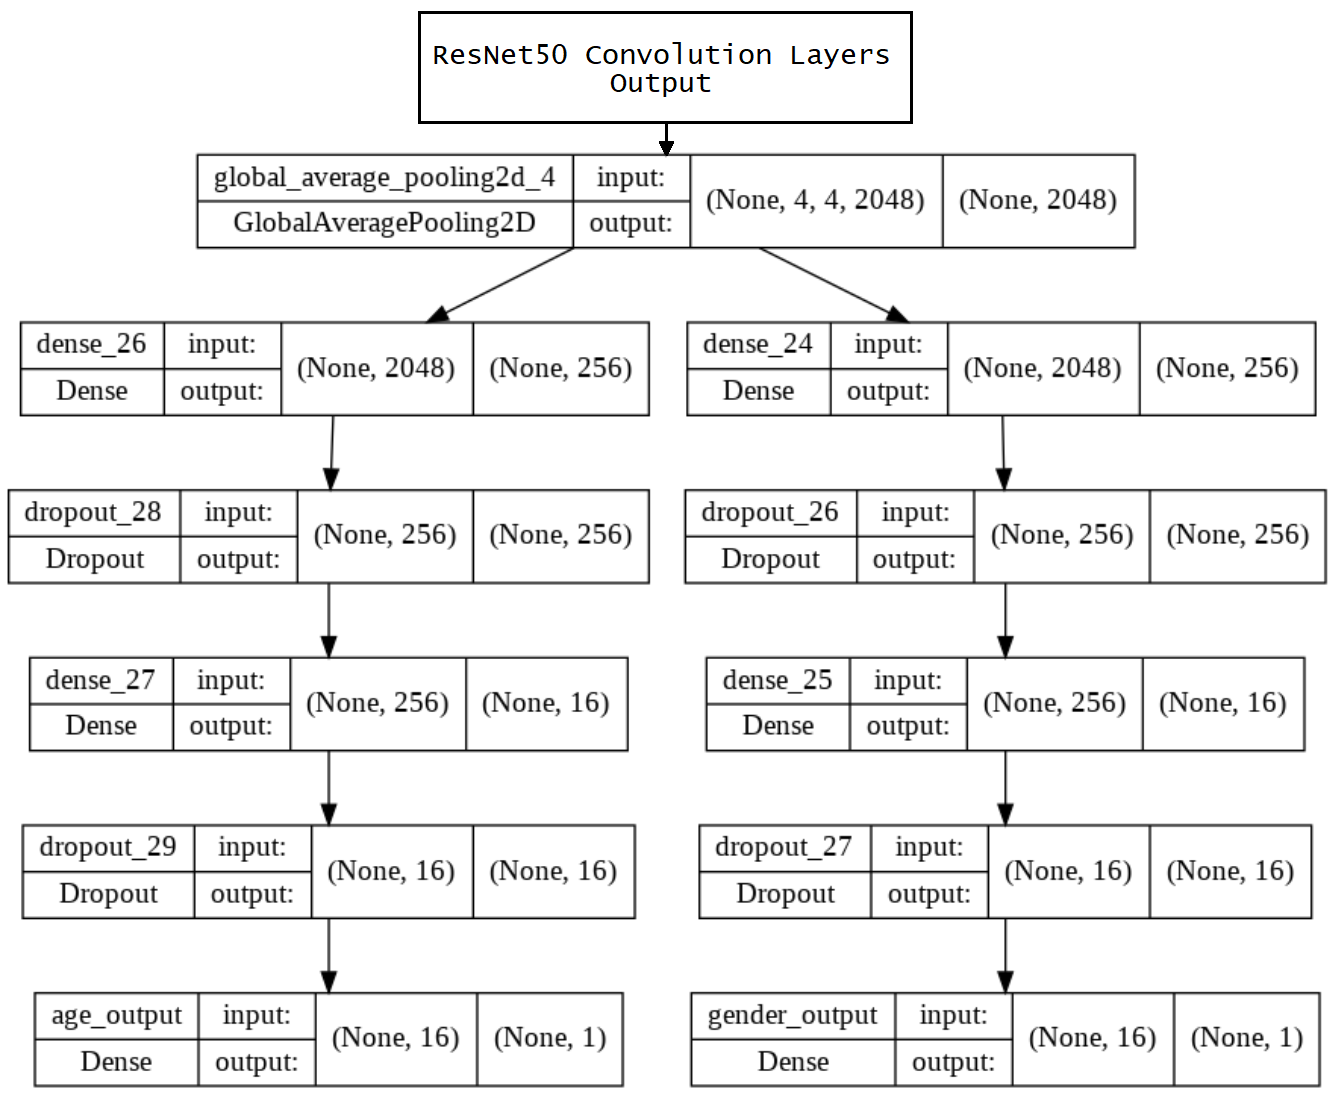
\includegraphics[height=0.5\textheight]{ModelBGraph_sample_simplified_dropouts_truncated.png}
\end{figure}
Following the ResNet output, we perform a global pool (rather than flatten as it didn't seem to learn) and created two FCN branches from this for the gender and age predictions.
Both branches utilised dropout weights.

Unfortunately we find the model started heavily over-fitting during training after a some number is epochs.
If left to train for longer it would continue to improve training accuracy, however validation would not, and occasionally get worse.
So as a form of hyper-parameter training we implemented a stop early callback which would end the training and retain the best weights (with respect to validation loss output) if the validation loss failed to improve over 3 epochs.

\subsubsection{Over-Fitting Prevention}


\subsection{Training}


\subsection{Performance}

